\documentclass{beamer}
\usepackage{amsmath}
\usepackage{amsfonts}
\usepackage{amssymb}
\usepackage{multicol}
\usepackage{float} %设置图片浮动位置的宏包
\usepackage{colortbl}
\usepackage{tabularx}
\usepackage{threeparttable}
\usepackage{booktabs}
\usepackage{setspace}
\usepackage{fontspec}
\usepackage{bm}
\usepackage{ctex} %汉语包
\usetheme{Madrid}
\usecolortheme{default}

\setCJKmainfont{STFangsong}


%初始化设置
%配色网站:https://mpetroff.net/files/beamer-theme-matrix/

\title{Do Corporations Retain Too Much Cash?}
\subtitle{——Evidence from a Natural Experiment}
\author{黄倪远\quad 秦子铉\quad 姚宗庆\quad 张嘉颢}
\institute{浙江大学}
\date{\today}

%封面设置

\setcounter{tocdepth}{2}

\begin{document}

\frame{\titlepage}

\begin{spacing}{1.2}
    \begin{frame}{目录}
      \begin{multicols}{3}
      \small{\tableofcontents[currentsection,sectionstyle=show/show]}
      \end{multicols}
    \end{frame}
\end{spacing}



%目录设置

\section{原文回顾}
\frame{
    \frametitle{基本信息与研究背景}

    \begin{itemize}
        \item
        2014年,为了激励企业增加投资,促进消费需求,韩国迅速提出并通过了对企业现金留存征收新税的税制计划。
        \vspace{0.2cm}
        \item
        \textbf{本文以此为背景,研究了“公司是否持有了过多现金”的问题。}\\
        具体来看,如果一家公司的现金持有量是最优的,那么外部冲击(导致其改变现金持有量)会减少Firm Value;如果如果一家公司的现金持有量是过多的,那么外部冲击会增加Firm Value。
    \end{itemize}
}

\frame{
    \frametitle{回归模型}

    \begin{itemize}
        \item
        为了研究新的税制计划对公司现金持有量的影响,作者建立了\textbf{DID模型},比较了新的税制计划生效受到影响的公司与未受影响的公司,时间为生效前两年(2013-2014)至改革后两年(2015-2016)。
        \item
        为了确定改革是否提高或降低了受影响公司的估值,作者关注\textbf{CAR(cumulative abnormal returns)变量},使用3天窗口期,从两个重大事件(草案发布,法规实施)的前一天到后一天捕捉公司层面的CAR变化。
        \vspace{0.2cm}
        \item
        研究发现经历过亚洲金融危机的企业在冲击后减少现金留存幅度、增加支出幅度、提升估值幅度更大;公司治理好与坏的公司在冲击后均减少了现金留存;公司治理差的公司提高了对外投资支出,但没有提升公司估值(因为新的投资没有正的NPV),而公司治理好的公司提高了payouts,提高了公司估值。
    \end{itemize}
}

\frame{
    \frametitle{机制提出与检验}

    \begin{itemize}
        \item
        作者提出并检验了两种使公司超额储备现金的机制,Behavioral biases与Agency conflicts。
        \vspace{0.3cm}
        \item
        \textbf{Behavioral biases机制}指出经历过经济危机的公司经理倾向于持有更多的现金,越看重经济危机的经历的就越是如此
        \item
        \textbf{Agency conflicts机制}则指出公司治理问题、代理人问题会导致持有更多的现金。
    \end{itemize}
}

\section{数据来源与数据处理}
\subsection{数据来源}
\frame{
    \frametitle{数据来源}

    \begin{itemize}
        \item
        \alert{复现中使用的数据主要由原文作者提供,经确认,这份数据为作者模拟得到,并非真实数据。}
        \item
        数据从DataGuide收集,并使用韩国公平贸易委员会(KFTC)每年制定的大型企业集团的数据来确定哪些公司属于财阀。
        \vspace{0.2cm}
        \item
        作者的数据经过一下筛选操作:
        \vspace{0.2cm}
        \begin{enumerate}
            \item 排除缺少账面资产数据的公司,缺少这项数据将导致没法判断公司属于控制组还是处理组;
            \item 排除金融公司和公用事业公司,因为这些公司的现金和投资政策受到监管;
            \item 排除极端数据,具体指总资产低于 10 亿韩元,一些资本支出低于总资产的 10 \% 的公司和现代汽车、起亚汽车和现代摩比斯三家公司(因为这三家公司在样本期间对房地产进行了大量投资,而这些投资在改革冲击之前就做好规划,与冲击无关)。
        \end{enumerate}
        \item
        最终样本中总共含20,916 家公司。
    \end{itemize}

}

\subsection{样本空间的构建}
\frame{
    \frametitle{样本空间的构建}

    \begin{itemize}
        \item<1->
        所有的回归模型均在下面三个样本空间中分别回归:
        \vspace{0.2cm}
        \begin{enumerate}
            \item 完整样本;
            \item 账面资产在 100 亿至 900 亿之间的样本;
            \item 在每个被处理公司和其最近的邻居之间进行一对一匹配的样本(在匹配过程中,我们要求在行业和公开上市地位上完全匹配,在这个集合中,我们根据改革前的销售额、销售增长、净收入和杠杆的马哈拉诺比斯距离来选择最近的邻居)。
        \end{enumerate}
    \end{itemize}

}

\section{描述性统计}
\frame{
    \frametitle{样本构成}

    \begin{center}
        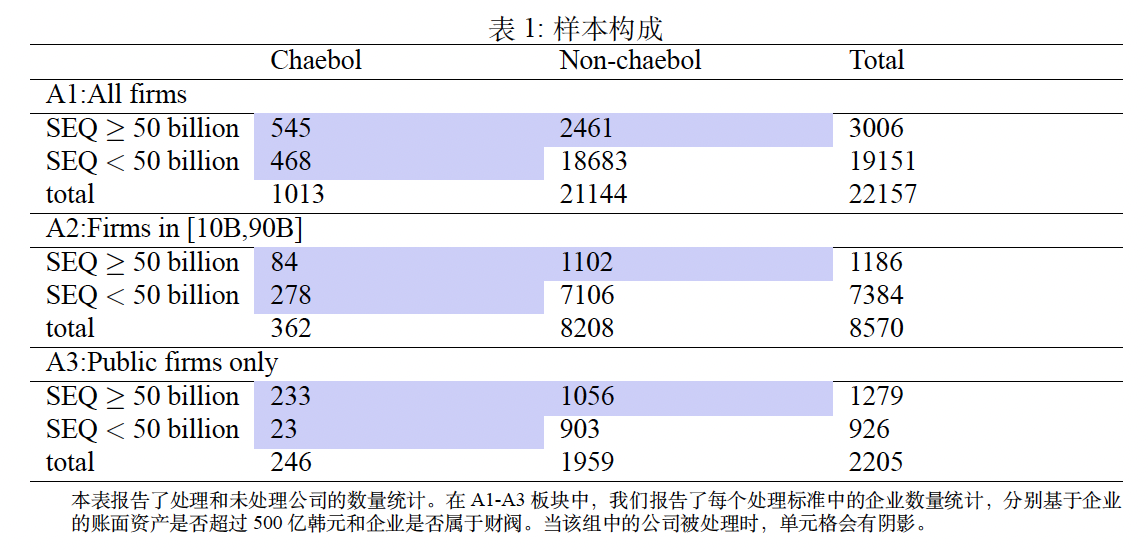
\includegraphics[scale=0.55]{表一.png}
    \end{center}
}

\frame{
    \frametitle{关键指标描述性统计}

    \begin{center}
        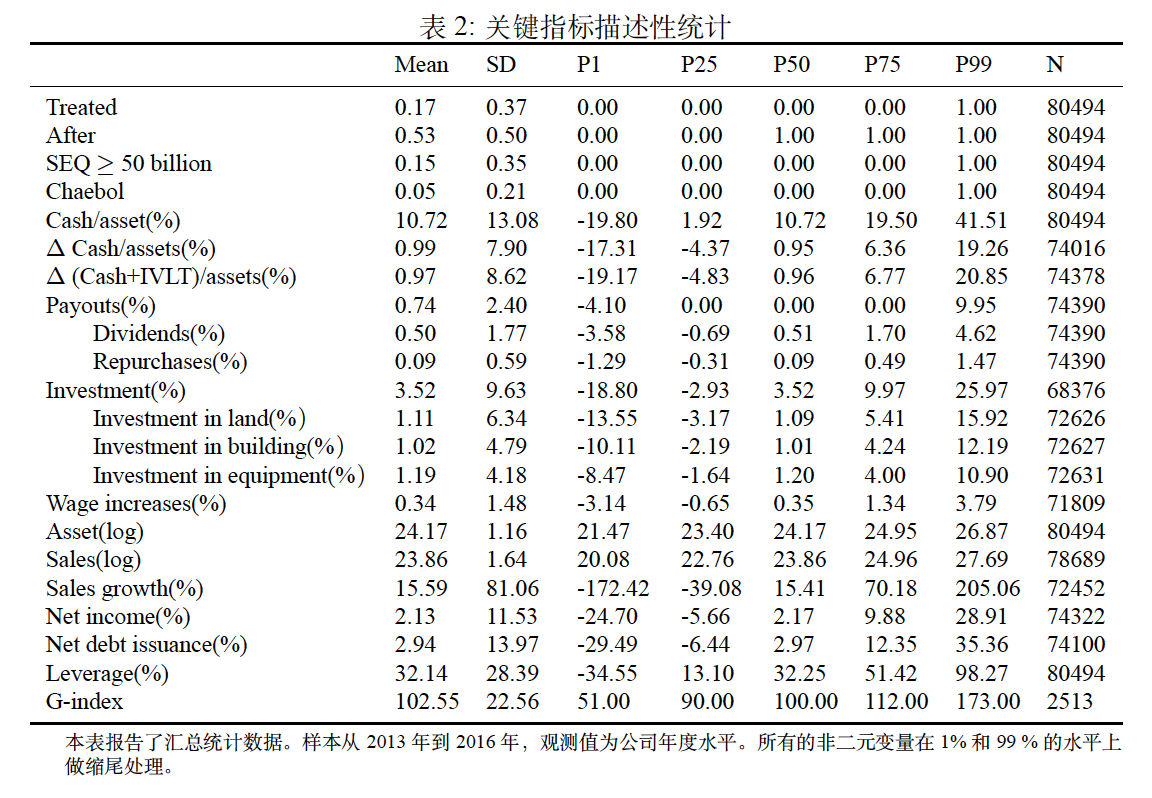
\includegraphics[scale=0.55]{表二.png}
    \end{center}
}

\section{回归分析}
\subsection{回归模型建立}
\frame{
    \frametitle{回归模型建立}

    \begin{itemize}
        \item 
        为了分析改革对企业财务和投资政策的影响,我们采用了差异分析法。该分析比较了改革前两年(2013-14 年)和改革后两年(2015-16 年)接受改革处理的公司和未接受改革处理的公司。我们估计以下基线模型:
        \vspace{0.2cm}
        \footnotesize{
        \begin{equation}
            y_{i, t}=\theta+\beta_{0} Treated _{i}+\beta_{1} After _{t}+\beta_{2} Treated _{i} \times After _{t}+\eta^{\prime} \cdot \mathbf{X}_{i, t}+\varphi_{i}+\tau_{t}+\psi_{j, t}+\varepsilon_{i, t}
        \end{equation}
        }
        \vspace{0.2cm}
        \indent 其中$i$代表公司,$j$ 代表行业,$t$ 代表年份。
        \begin{center}
            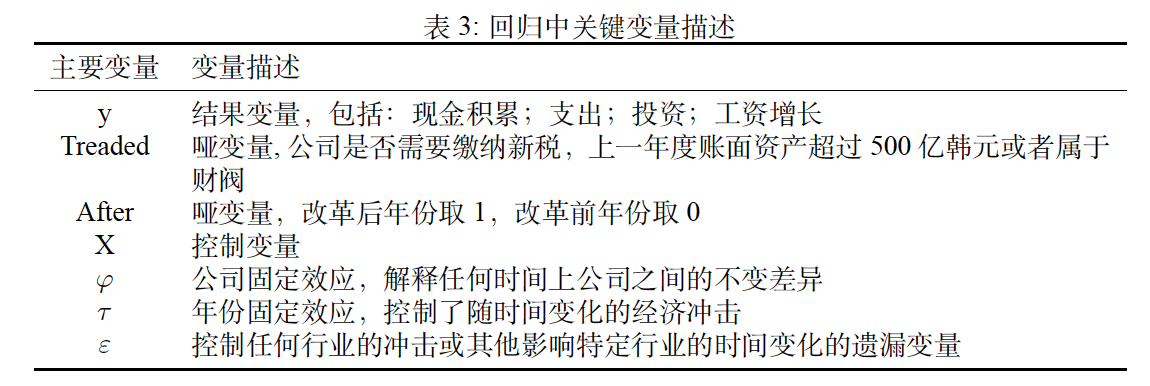
\includegraphics[scale=0.55]{表三.png}
        \end{center}
    \end{itemize}
}  

\subsection{对现金留存的影响}
\frame{
    \frametitle{对现金留存的影响}

    \begin{itemize}
        \item
        该部分验证改革会使得处理组的公司保留更少的现金。
        \begin{center}
            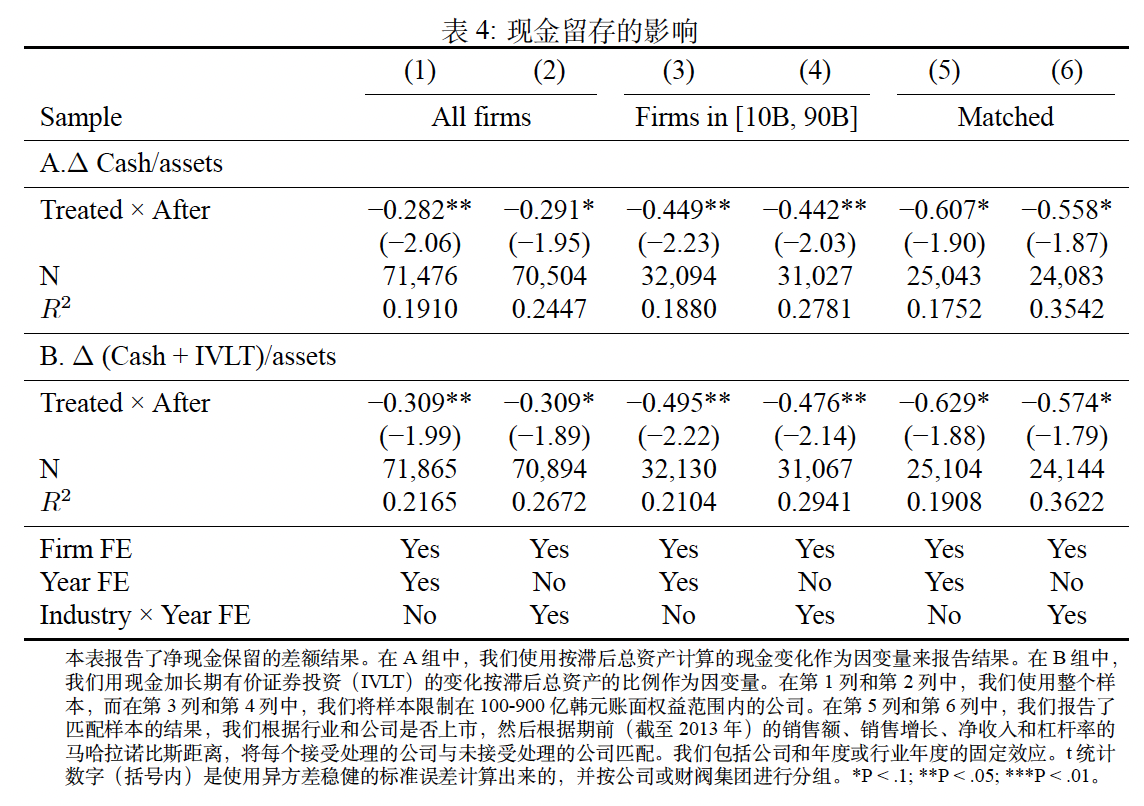
\includegraphics[scale=0.5]{表四.png}
        \end{center}
    \end{itemize}
}

\subsection{现金的边际价值}
\frame{
    \frametitle{现金的边际价值}

    \begin{itemize}
        \item
        原先持有一美元现金的价值小于一美元,而改革政策会使这个边际价值增加,增加到接近一美元。
        \scriptsize{
        \begin{equation}
            \begin{split}
                \text { Excess Return }_{i, t}= &\theta+\beta_{1} \Delta \text { Cash }_{i, t}+\beta_{2} \text { Treated }_{i}+\beta_{3} \text { After }_{t}+\beta_{4} \text { Treated }_{i} \times \text { After }_{t} \\
                &+\beta_{5} \Delta \text { Cash }_{i, t} \times \text { Treated }_{i}+\beta_{6} \Delta \text { Cash }_{i, t} \times \text { After }_{t} \\ &+\beta_{7} \Delta \text { Cash }_{i, t} \times \text { Treated }_{i} \times \text { After }_{t}+\eta^{\prime} \cdot \mathbf{X}_{i, t}+\varepsilon_{i, t} \\  
            \end{split}
        \end{equation}
        }
    \end{itemize}
}

\frame{
    \frametitle{现金的边际价值}

    \begin{itemize}
        \item
        原先持有一美元现金的价值小于一美元,而改革政策会使这个边际价值增加,增加到接近一美元。
        \begin{center}
            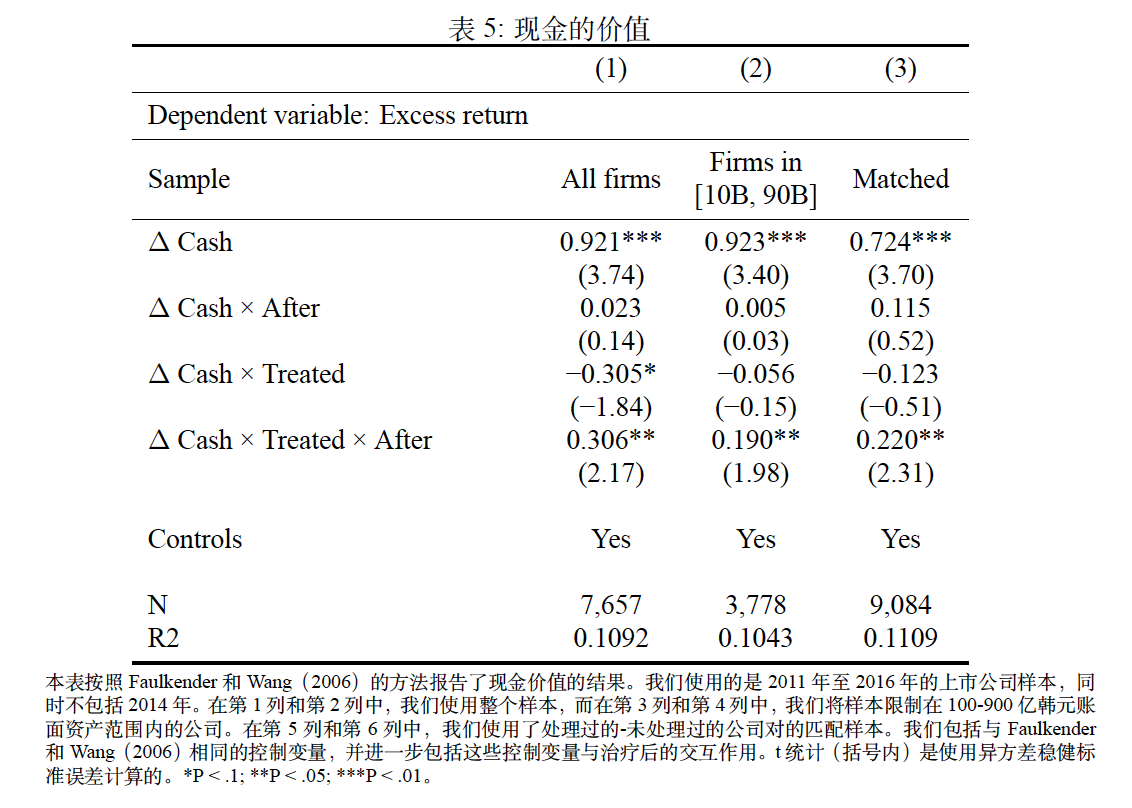
\includegraphics[scale=0.5]{表五.png}
        \end{center}
    \end{itemize}
}

\subsection{边际现金的其他用途:对于报酬、投资和工资的影响}
\frame{
    \frametitle{边际现金的其他用途:对于报酬、投资和工资的影响}

    \begin{itemize}
        \item
        在改革之后,公司会增加对报酬、投资和工资三个方面都有明显增长。
        \vspace{-0.4cm}
        \begin{center}
            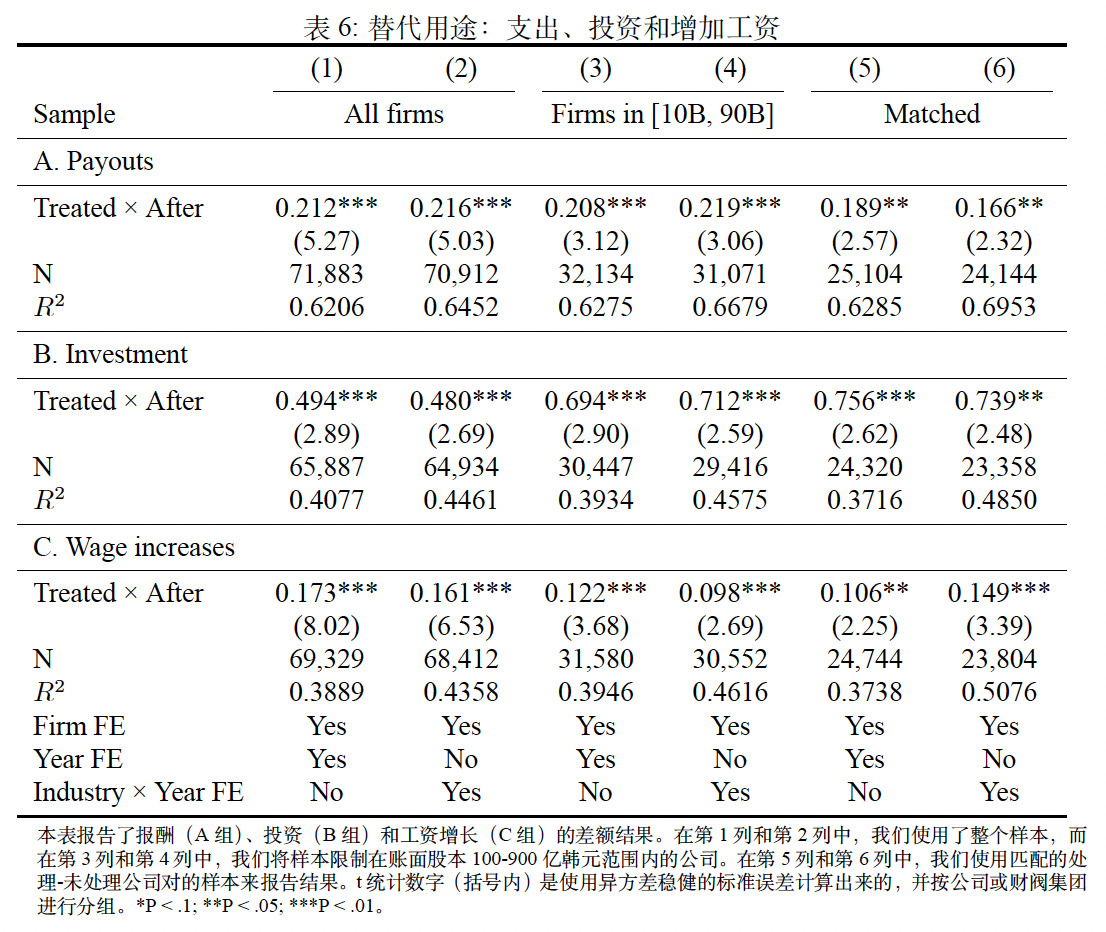
\includegraphics[scale=0.46]{表六.png}
        \end{center}
    \end{itemize}
}

\subsection{渠道分析}
\subsubsection{拥有危机记忆的公司对于改革的影响}
\frame{
    \frametitle{拥有危机记忆的公司对于改革的影响}

    \begin{itemize}
        \item
        有危机记忆的受处理企业在改革后更多地减少了现金保留,这些企业也更多地提高了报酬、投资和工资。
        \vspace{0.2cm}

        \tiny{
        \begin{equation}
            \begin{split}
                y_{i, t}=&\theta+\beta_{0} \text { Treated }_{i}+\beta_{1} \text { After }_{t}+\beta_{2} \text { Treated }_{i} \times \text { After }_{t}+\beta_{3} \text { Treated }_{i} \times \text { CrisisMemory }_{i} \\ &+\beta_{4} \text { CrisisMemory }_{i} \times \text { After }_{t}+\beta_{5} \text { Treated }_{i} \times \text { CrisisMemory }_{i} \times \text { After }_{t} \\ &+\varphi_{i}+\tau_{t}+\psi_{j, t}+\varepsilon_{i, t} 
            \end{split}
        \end{equation}
        }
    \end{itemize}
}

\subsubsection{公司治理对于改革的影响}
\frame{
    \frametitle{公司治理对于改革的影响}

    \begin{itemize}
        \item
        治理好的公司和治理差的公司在现金保留的反应上没有显著差异。但是对于现金的分配上有着不同。治理好的公司会增加支付,减少投资和工资支付。
        \begin{center}
            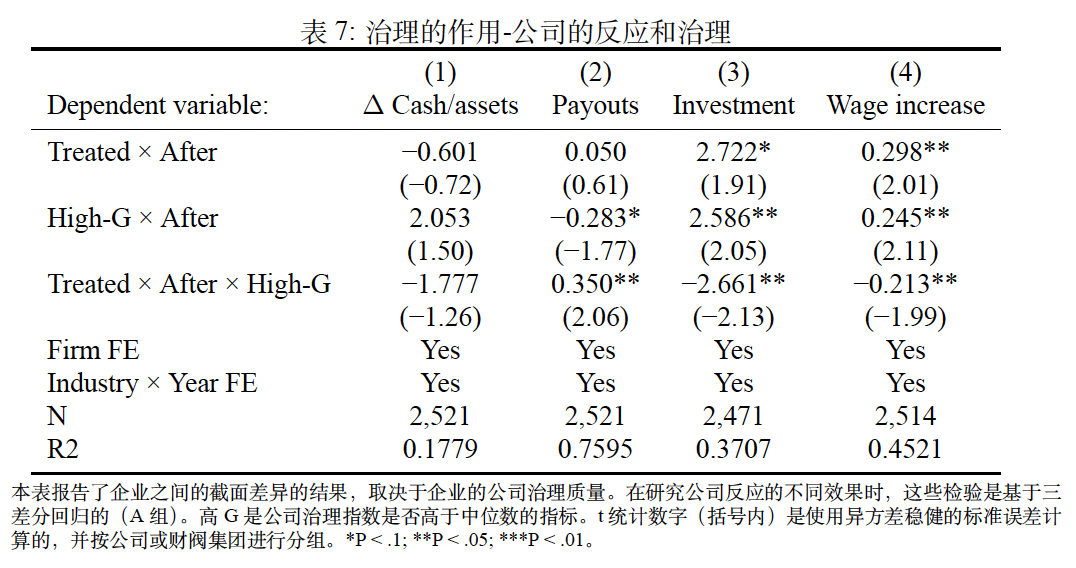
\includegraphics[scale=0.55]{表七.png}
        \end{center}
    \end{itemize}
}

\section{稳健性检验}
\subsection{平行趋势检验}
\frame{
    \frametitle{平行趋势检验}

    \begin{itemize}
        \item
        为了进一步支持平行趋势的假设,我们报告了改革前几年受处理和未受处理企业之间主要结果变量的前趋势结果。
        \begin{center}
            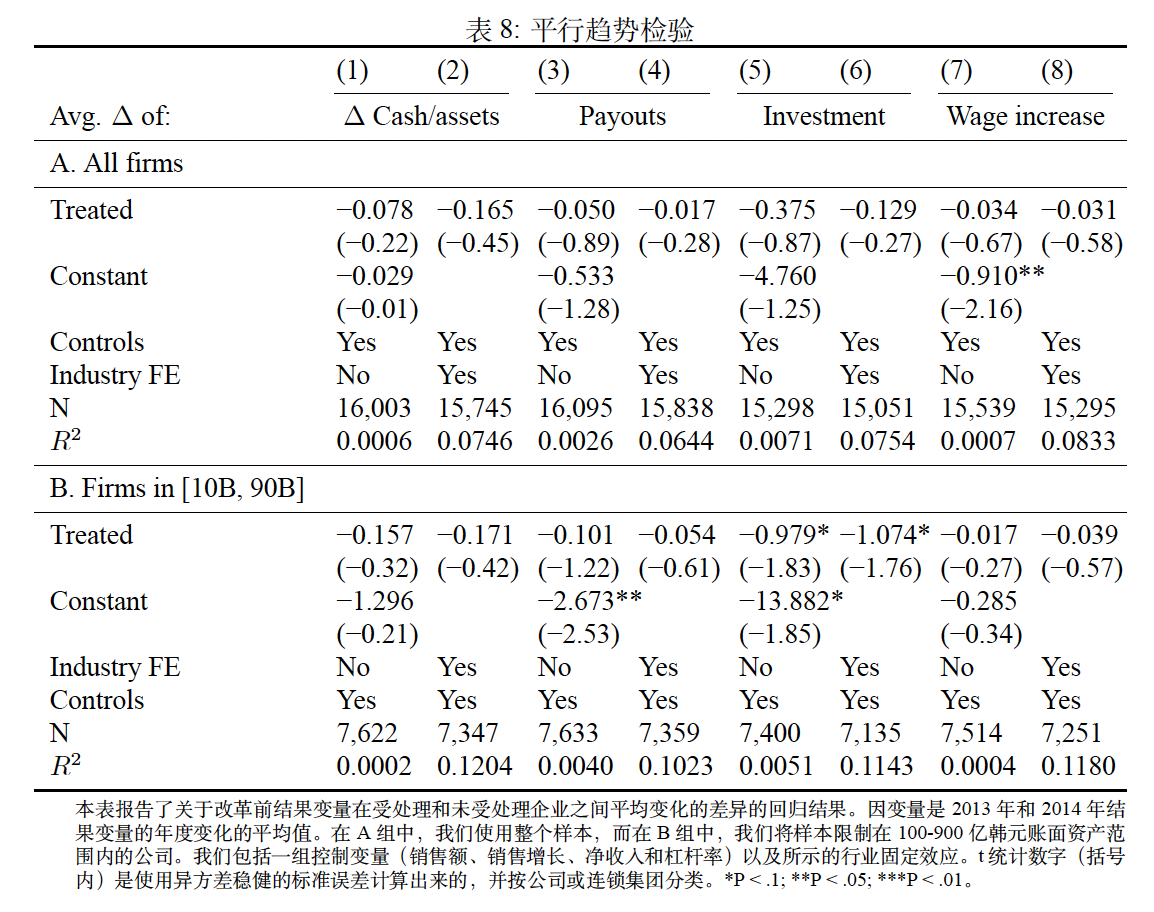
\includegraphics[scale=0.45]{表八.png}
        \end{center}
    \end{itemize}
}

\subsection{排除财阀}
\frame{
    \frametitle{排除财阀}

    \begin{itemize}
        \item
        我们在测试中排除了所有的财阀企业。对于剩下的那些非财阀公司,一个公司是否被处理完全取决于其账面资产是否高于或低于500亿韩元。我们进一步将样本限制在100-900亿韩元的范围内。在这些测试中,结果仍然与我们之前的基线研究结果相似,这意味着\textbf{财阀公司和非财阀公司之间任何可能的趋势差异都不会驱动之前的结果。}
    \end{itemize}
}

\subsection{安慰剂检验}
\frame{
    \frametitle{安慰剂检验}

    \begin{itemize}
        \item
        在改革宣布之前,人们可能已经存在预期,认为财阀会受到这种改革的影响,而积极的宣布效应可能反映了这些公司的监管不确定性的某种解决。
        \begin{center}
            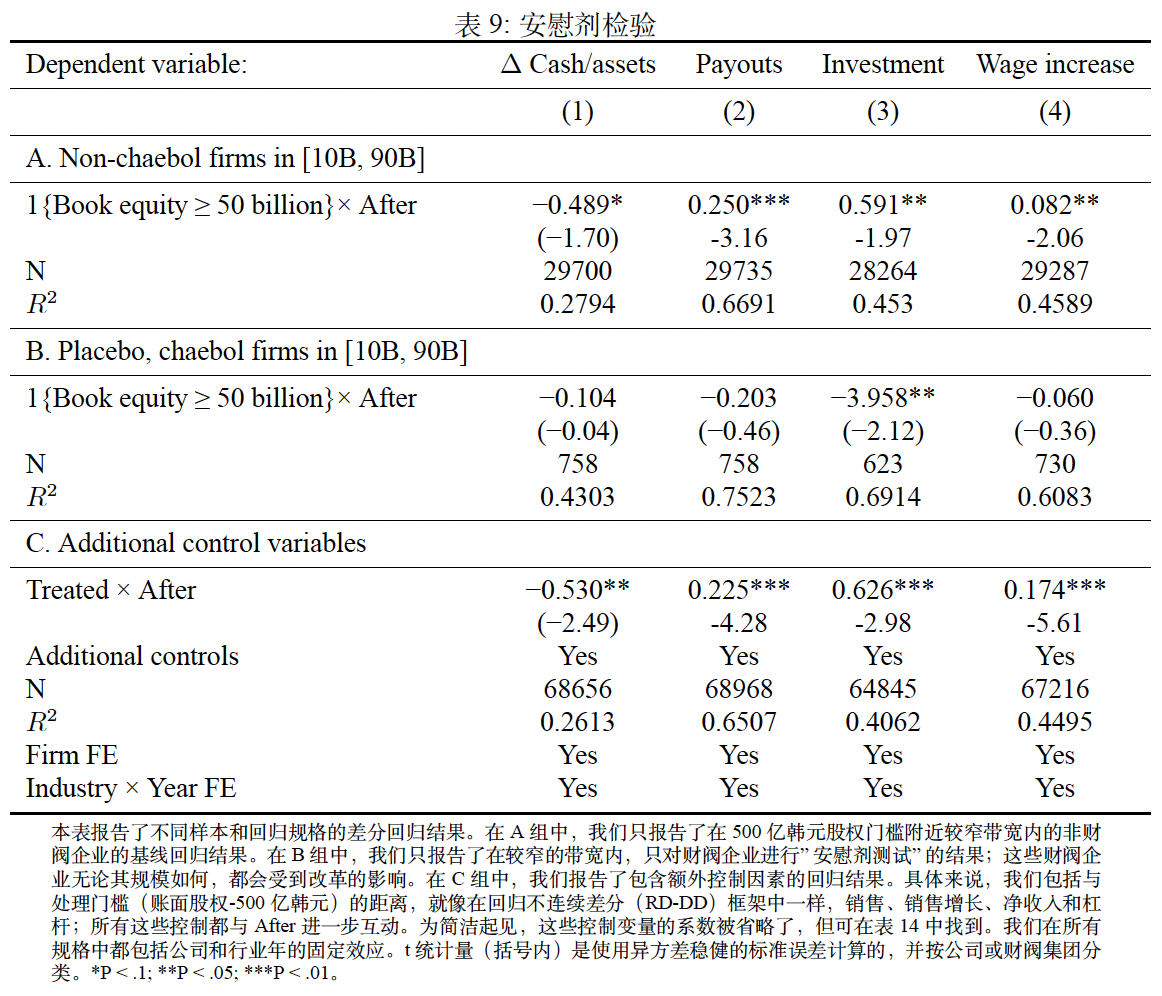
\includegraphics[scale=0.38]{表九.png}
        \end{center}
    \end{itemize}
}

\subsection{额外控制}
\frame{
    \frametitle{额外控制}

    \begin{itemize}
        \item
        我们在基线回归中加入了与After 相互作用的距离阈值(账面权益-500 亿韩元)的控制。结果表明在考虑到与门槛的距离和其他可能的协变量时,估计的效果仍然相似或变得更强。
        \begin{center}
            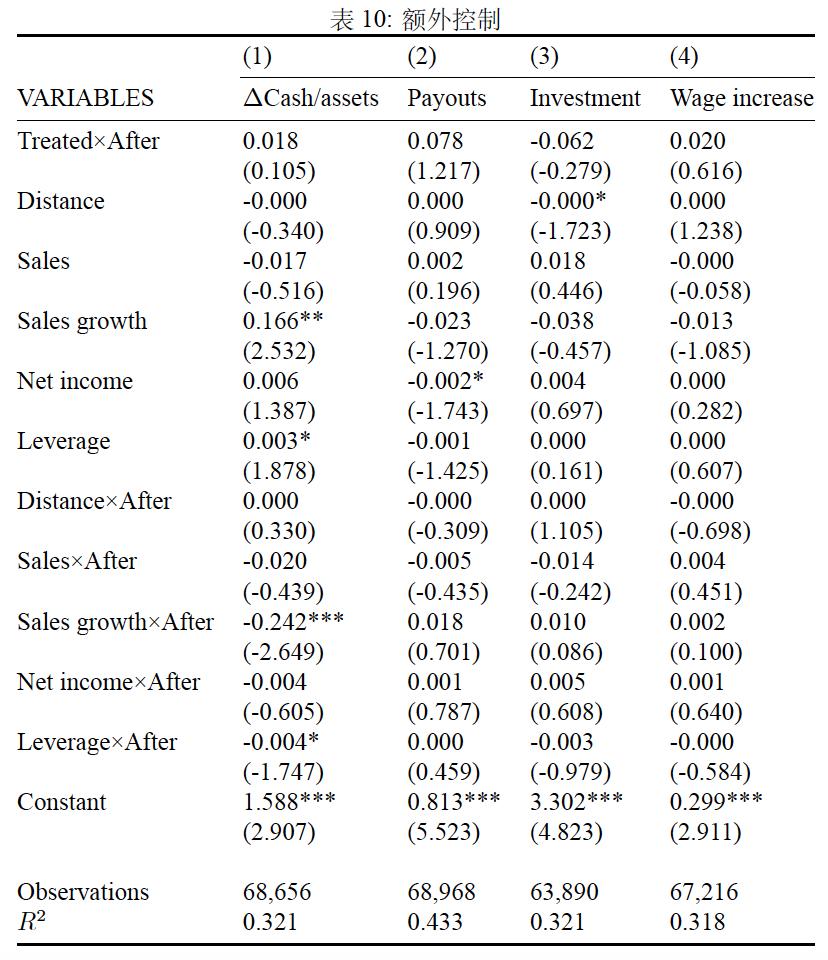
\includegraphics[scale=0.38]{表十.png}
        \end{center}
    \end{itemize}
}

\subsection{避免公司主动调整账面价值来避税的可能}
\frame{
    \frametitle{避免公司主动调整账面价值来避税的可能}

    \begin{itemize}
        \item
        我们使用”Donut RD ” 的实证策略重新估计我们的结果,即我们专注于100-900 亿韩元的范围,但不包括450-550 亿韩元的公司,对这些公司来说,缩小规模以避免纳税的动机可能是最强烈的。
        \vspace{0.2cm}
        \begin{center}
            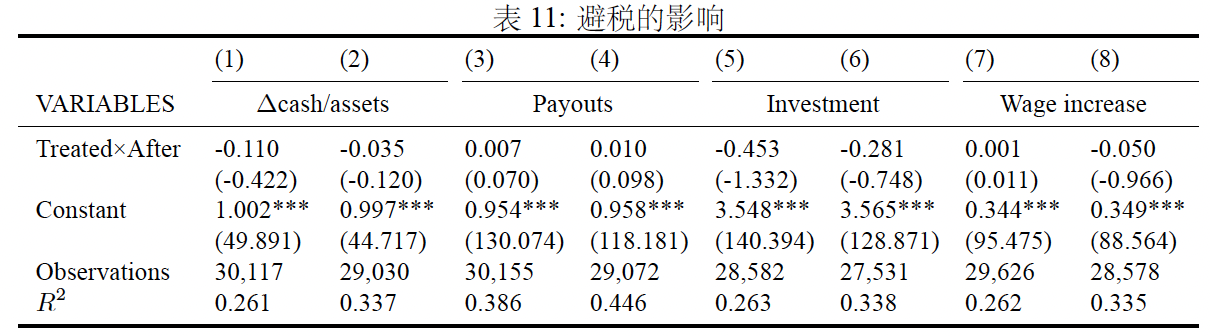
\includegraphics[scale=0.5]{表十一.png}
        \end{center}
    \end{itemize}
}

\section{本土研究拓展}
\subsection{研究回顾}
\subsubsection{研究背景}
\frame{
    \frametitle{本土文献研究背景}

    \begin{itemize}
        \item
        税收中性原则指国家征税以不干预市场经济运行,平等对待一切纳税人为目标的税收制度。\textbf{我国曾经的增值税转嫁规律及可抵扣范围设计导致留抵税款积压,给企业带来了资金困境、扭曲了税收中性原则。}
        \vspace{0.2cm}
        \item 为了改变这种扭曲,2018年6月,财政部联合国家税务总局颁布《关于2018年退还部分行业增值税留抵税额有关税收政策的通知》,对装备制造等先进制造业、研发等现代服务业等18个大类行业及电网企业期末留抵税额予以退还。
    \end{itemize}
}

\subsubsection{理论分析与研究假设}
\frame{
    \frametitle{理论分析与研究假设}

    \begin{itemize}
        \item
        \textbf{假设1:}留抵退税政策有助于降低试点企业的现金持有。
        \vspace{0.2cm}
        \item
        \textbf{假设2:}“资源效应”和“信号效应”的共同作用将对极端持现的企业影响更大。
        \vspace{0.2cm}
        \item
        \textbf{假设3:}相比衰退期企业,留抵退税政策对成长期、成熟期企业的现金持有影响更大。
        \vspace{0.2cm}
        \item
        \textbf{假设4:}相比于其他纳税信用等级企业,留抵退税政策对纳税信用等级高的企业现金持有的影响更大。
    \end{itemize}
}

\subsubsection{异质性分析}
\frame{
    \frametitle{异质性分析}

    \begin{itemize}
        \item
        \textbf{作者还在“资源效应”与“信号效应”层面进行了异质性分析。}发现在留抵税款规模和融资约束层面,积压留抵税额规模更大、融资约束越严重的企业现金持有下降更显著;在税负转嫁能力和市场竞争能力层面,税负转嫁能力和市场竞争能力较弱的企业现金减持更为显著;税收征管力度越强、环境不确定性越高、环境动态性越高、环境丰富性越高的企业现金持有下降越显著。
        \vspace{0.2cm}
        \item
        在研究留抵退税政策对企业极端持现金的影响时,作者建立了分位数回归模型。回归结果显示\textbf{相比于现金持有较为“平均”的企业,留抵退税政策对于现金持有极高的企业以及现金持有极低的企业影响更大。}
    \end{itemize}
}

\subsubsection{政策效果检验}
\frame{
    \frametitle{政策效果检验}

    \begin{itemize}
        \item
        作者运用现金流模式法将样本企业划分为成长期、成熟期和衰退期,探究留抵退税政策对不同生命周期阶段的企业持现影响。结果显示,\textbf{相比于衰退期企业,留抵退税政策对成长期企业和成熟期企业现金持有的影响更大。}
        \vspace{0.2cm}
        \item
        作者还根据国家税务总局提供的纳税信用等级进行分组分析,结果显示\textbf{相比于其他纳税信用等级企业,留抵退税政策对纳税信用等级A级企业现金持有的影响更大。}
    \end{itemize}
}

\subsubsection{经济后果检验}
\frame{
    \frametitle{经济后果检验}

    \begin{itemize}
        \item
        作者从短期经营绩效、经营风险波动视角分析留抵退税政策冲击下企业持现调整的经济后果。研究发现留抵退税政策下企业持现调整对于企业短期绩效产生了正向促进作用,对于企业经营业绩波动带来改善,且上述影响均对于资本密度高的企业影响更为显著。
    \end{itemize}
}

\subsection{研究设计}
\subsubsection{样本选择}
\frame{
    \frametitle{样本选择}

    \begin{itemize}
        \item
        以财税[2018]70号文的颁布作为改善增值税税收中性的外生冲击,选取2013-2020年全部A股上市公司作为研究的初始样本。
        \item
        作者的数据经过一下筛选操作:
        \vspace{0.2cm}
        \begin{enumerate}
            \item 删除样本期间IPO年度、挂牌ST以及退市样本;
            \item 删除金融行业样本;
            \item 删除关键变量数据确实及利润率、资产负债率异常样本;
            \item 用线性插值法对剩余样本中的缺失值进行填充;
            \item 对相关连续变量在1\%和99\%的水平上进行缩尾处理避免异常值影响。最终获得36232个“公司-年度”样本,涉及4529家公司。
        \end{enumerate}
        \vspace{0.2cm}
        相关数据主要来自wind数据库。
        \vspace{0.2cm}
        \begin{center}
            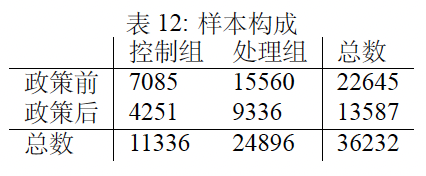
\includegraphics[scale=0.6]{表十二.png}
        \end{center}
    \end{itemize}
}

\subsubsection{模型设计与变量定义}
\frame{
    \frametitle{模型设计与变量定义}

    \begin{itemize}
        \item \textbf{我们采用双重差分法验证留抵退税政策对企业现金持有的影响。}依据财税[2018]70号文,将先进制造业、服务业等18个大类行业及电网企业作为处理组,以2018年作为政策时点。通过处理组与控制组在留抵退税政策前后时间趋势上的差异评估留抵退税政策的净效应。同时,控制年度和公司固定效应,具体为:
        \footnotesize{
        \begin{equation}
            cashhold _{i, t}=\beta_{0}+\beta_{1} treat _{i} \times post _{t}+\sum controls _{i, t}+\sum firm _{i}+\sum year _{t}+\varepsilon_{i, t}
        \end{equation}
        }
    \end{itemize}
}

\frame{
    \frametitle{变量定义}

    \begin{center}
        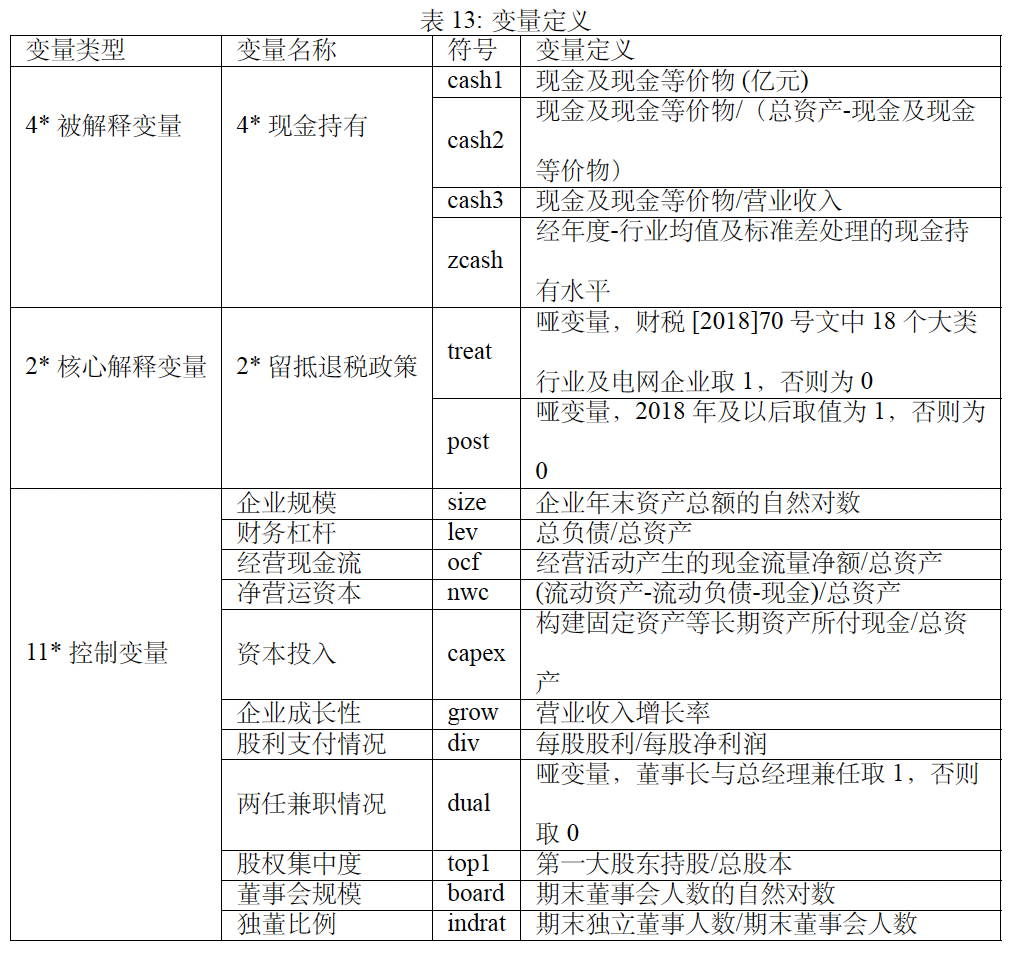
\includegraphics[scale=0.47]{表十三.png}
    \end{center}
}

\subsection{实证检验结果}
\subsubsection{全样本描述性统计}
\frame{
    \frametitle{全样本描述性统计}

    \begin{center}
        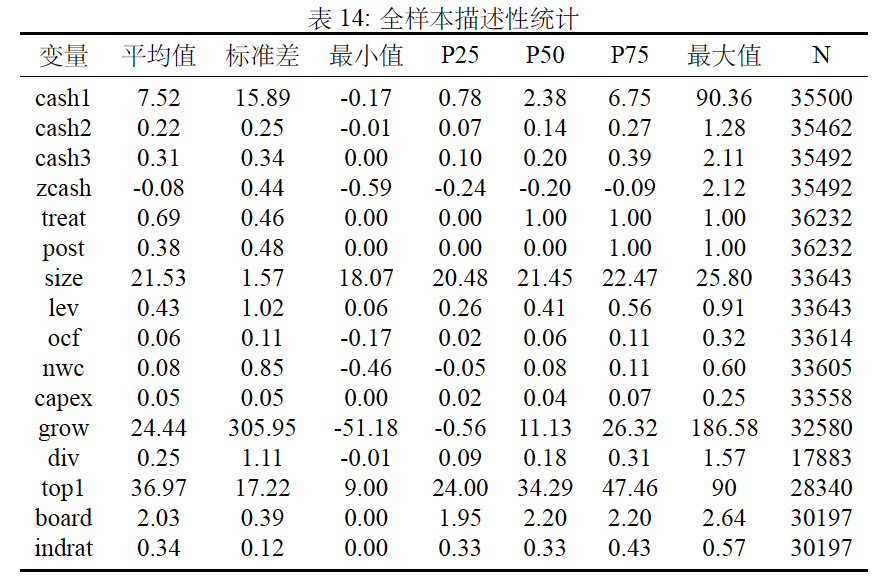
\includegraphics[scale=0.6]{表十四.png}
    \end{center}
}

\subsubsection{分组描述性统计}
\frame{
    \frametitle{分组描述性统计}

    \begin{center}
        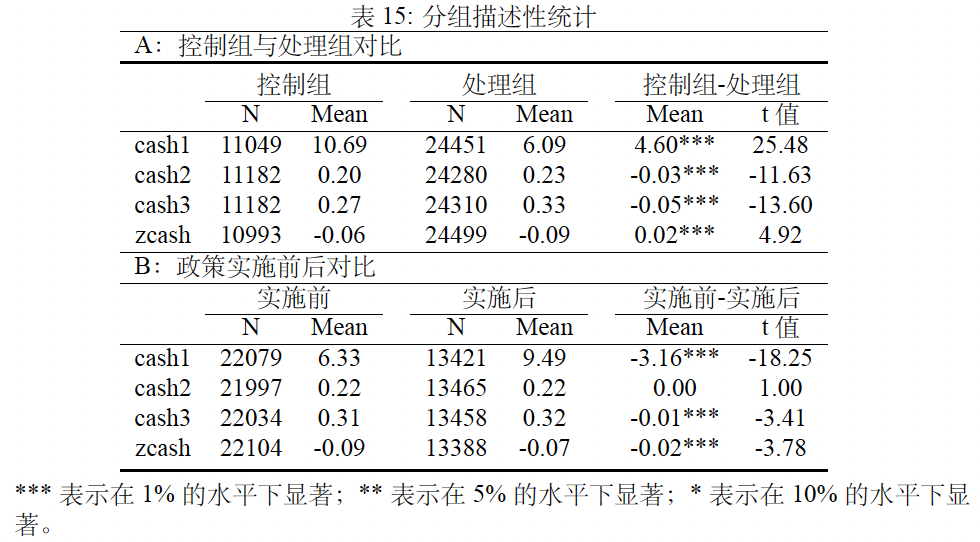
\includegraphics[scale=0.6]{表十五.png}
    \end{center}
}

\subsubsection{基准回归检验}
\frame{
    \frametitle{基准回归检验}

    \begin{itemize}
        \item
        基准回归结果如下表所示:
        \vspace{0.2cm}
        \begin{center}
            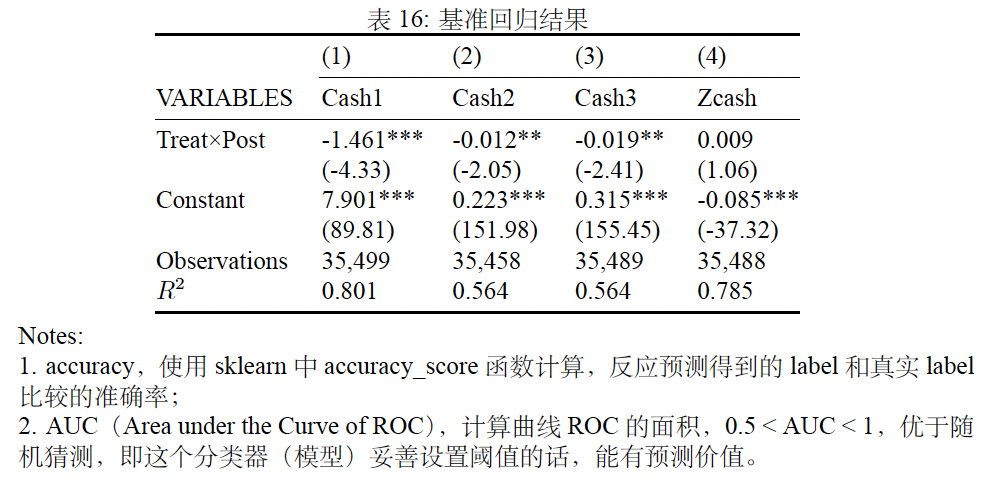
\includegraphics[scale=0.6]{表十六.png}
        \end{center}
    \end{itemize}
}

\subsection{平行趋势检验及稳健性检验}
\subsubsection{平行趋势检验} 
\frame{
    \frametitle{平行趋势检验}

    \begin{itemize}
        \item
        为了进一步支持平行趋势的假设,我们报告了改革前几年受处理和未受处理企业之间主要结果变量的前趋势结果。
        \begin{center}
            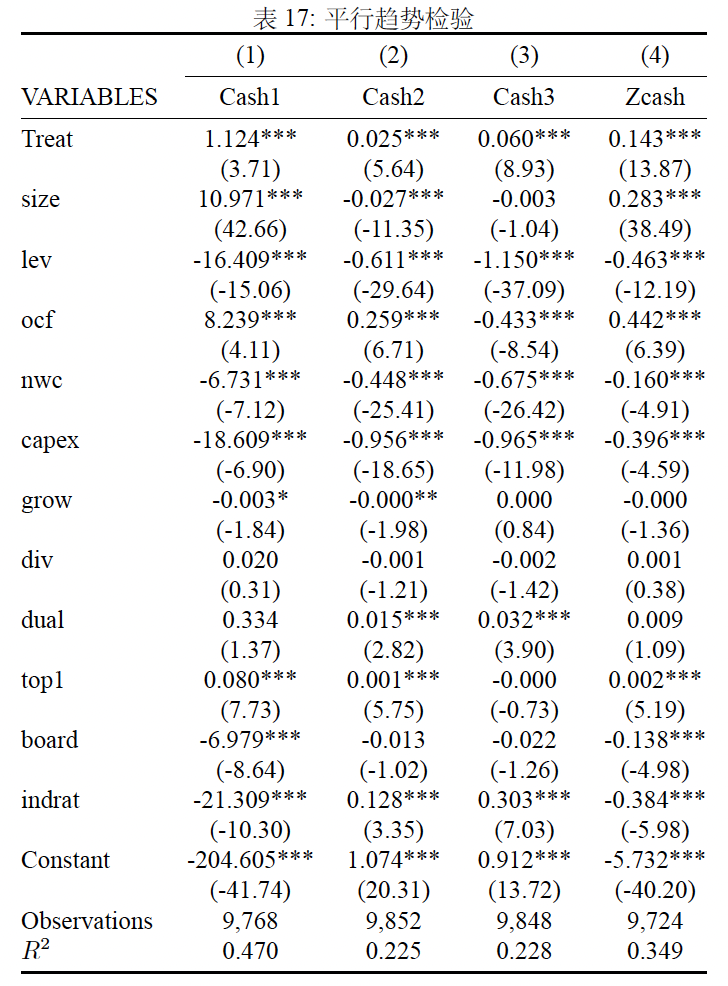
\includegraphics[scale=0.41]{表十七.png}
        \end{center}
    \end{itemize}
}

\subsubsection{稳健性检验:增加控制变量}
\frame{
    \frametitle{稳健性检验:增加控制变量}

    \begin{itemize}
        \item
        我们发现,在加入这一系列变量之后,结论变得更加显著。
        \begin{center}
            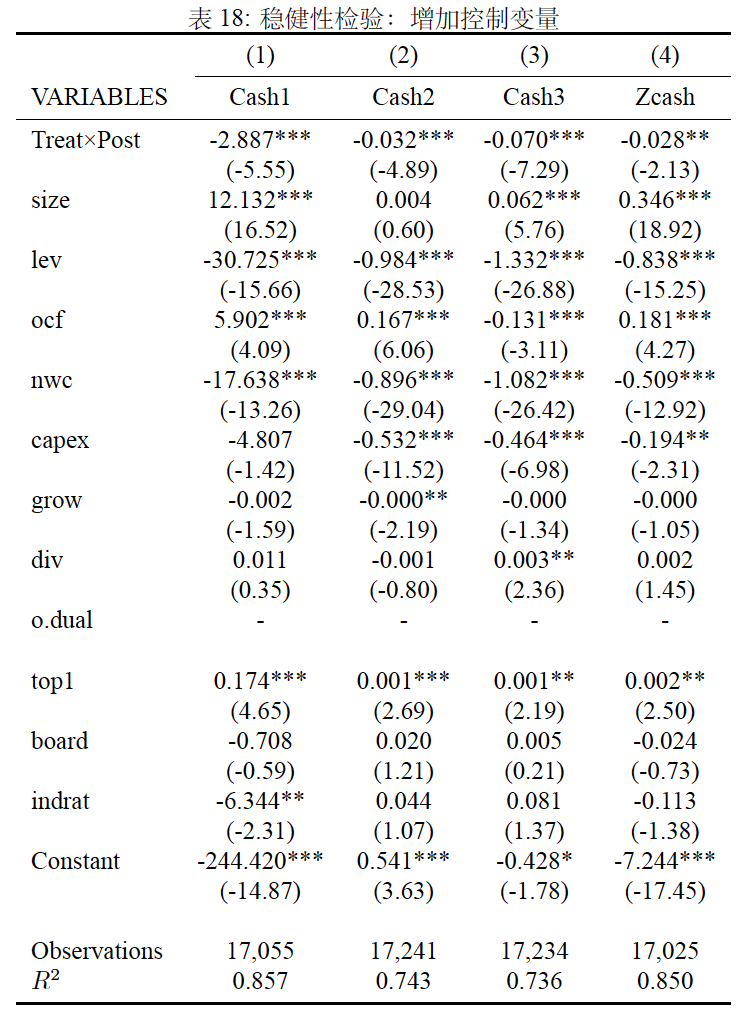
\includegraphics[scale=0.42]{表十八.png}
        \end{center}
    \end{itemize}
}
\section{结论}
\frame{
    \frametitle{结论}

    \begin{itemize}
        \item
        原文研究表明,\textbf{全球公司存在一定的“囤积”现金的现象},并以韩国样本探讨了如果企业保留较少的现金并在股息、工资或新投资上支出更多时,这些资金是否可以投入到更具生产力的用途,以及市场对此做出的反应。
    \end{itemize}
}

\frame{
    \frametitle{结论}

    \begin{itemize}
        \item
        原文通过利用韩国一项对现金留存征收新税来遏制公司现金积累的税收改革,来构造自然实验调查该问题。
        \vspace{0.2cm}
        \item \textbf{平均而言,受改革影响的企业减少了现金留存,并在股息、工资增长和投资上支出更多。}在判断保留较少现金是否为更优决策时,需要考虑改革前受影响企业的现金及投资政策是否已经处于最优状态,以及现金留存替代用途的支出效益如何。
        \vspace{0.2cm}
        \item \textbf{改革后的市场对此的反应是积极的}(体现在企业估值的提高),这意 味着投资者预期企业的回应行为足够提高价值,以抵消因支付更高税收而产生的任何直接负面估值后果。这些结果与改革前企业现金留存过多的假设相一致。
    \end{itemize}
}

\frame{
    \frametitle{结论}

    \begin{itemize}
        \item
        在机制分析层面,原文从行为偏差和代理冲突来进行解释。
        \vspace{0.2cm}
        \item 从行为偏差角度来说,经历过金融危机的企业管理者倾向于在改革前持有更多现金,但这些企业在改革发生后也通过大幅削减现金留存作出了更强烈的回应,投资者的反应也更积极。
        \vspace{0.2cm}
        \item 从代理冲突的视角来看,改革前治理较弱的企业往往持有较多现金。然而,在改革之后,这些治理不佳的企业并未增加股息支付。相反,它们更倾向于将留存的现金分配给投资,导致相对较低的估值,这一现象与帝国建设理论相符。
        \vspace{0.2cm}
        \item 因此,一个重要的启示是,\textbf{使用政策杠杆来阻止企业保留过多的现金并非一定有效},因为具体企业的价值影响将取决于企业之所以保留如此多现金的原因以及它们如何将这些资金分配给替代用途。
    \end{itemize}
}

\frame{
    \begin{center}
        \Huge{Thank you}!
    \end{center}
}
\end{document}

